\subsection{Modellazione dei casi d'uso}
    \begin{flushleft}
        Qui viene riportato lo Use Case Diagram relativo all'applicazione, che per rendere la lettura più semplificata è stato diviso in più sezioni.
    \end{flushleft}
    
    \begin{figure}[H]
        \centering
        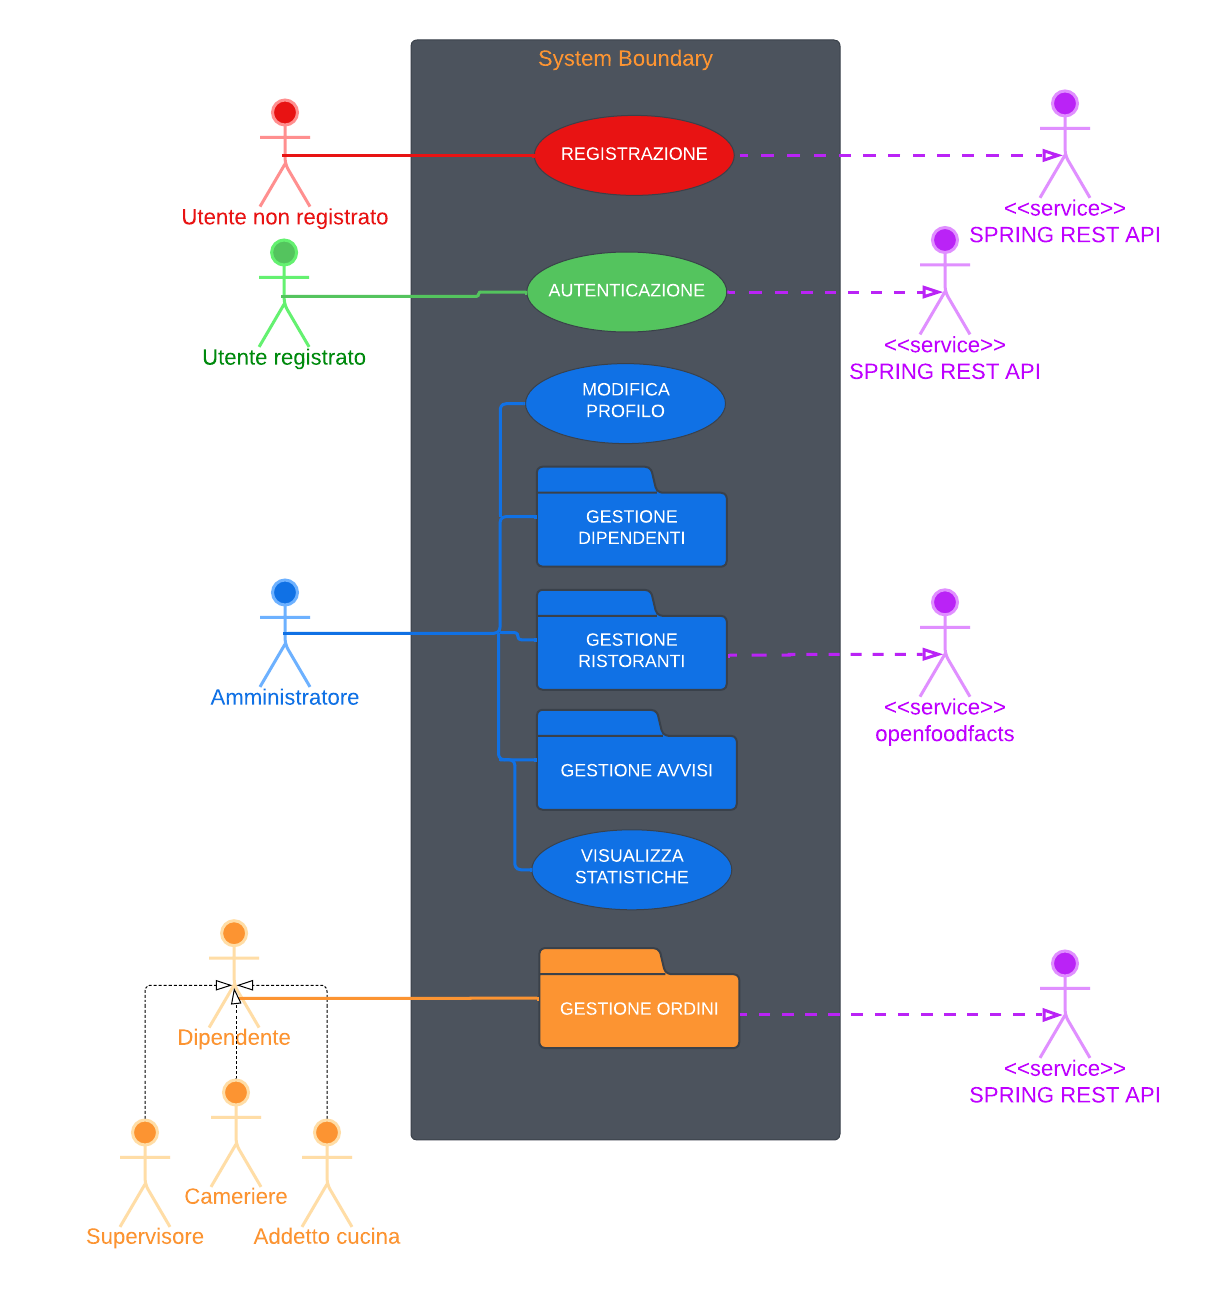
\includegraphics[width=0.8\textwidth]{assets/diagrammi/Use-Case/Use-Case Generale.png}
        \caption{Use Case dell'applicazione}
        \label{fig:ucdGenerale}
    \end{figure}
    
    \begin{figure}[H]
        \centering
        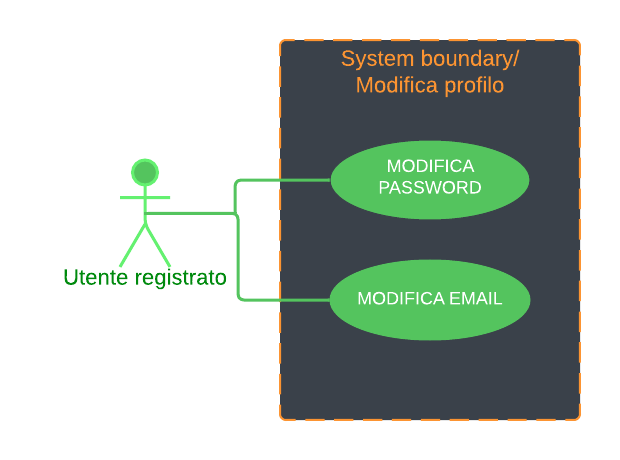
\includegraphics[width=0.8\textwidth]{assets/diagrammi/Use-Case/Modifica Profilo.png}
        \caption{Use Case relativo alla modifica del profilo}
        \label{fig:ucdModProfile}
    \end{figure}

    \begin{figure}[H]
        \centering
        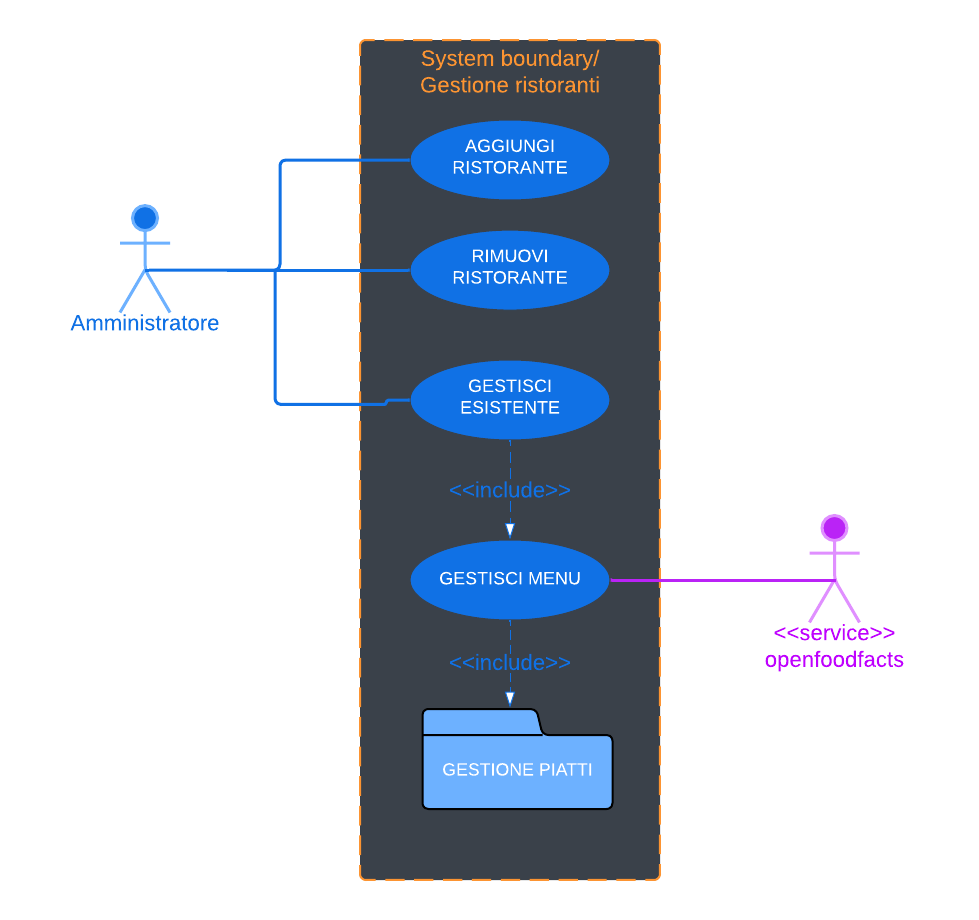
\includegraphics[width=0.8\textwidth]{assets/diagrammi/Use-Case/Gestione ristoranti.png}
        \caption{Use Case relativo alla gestione dei ristoranti}
        \label{fig:ucdResturantMgmt}
    \end{figure}

    \begin{figure}[H]
        \centering
        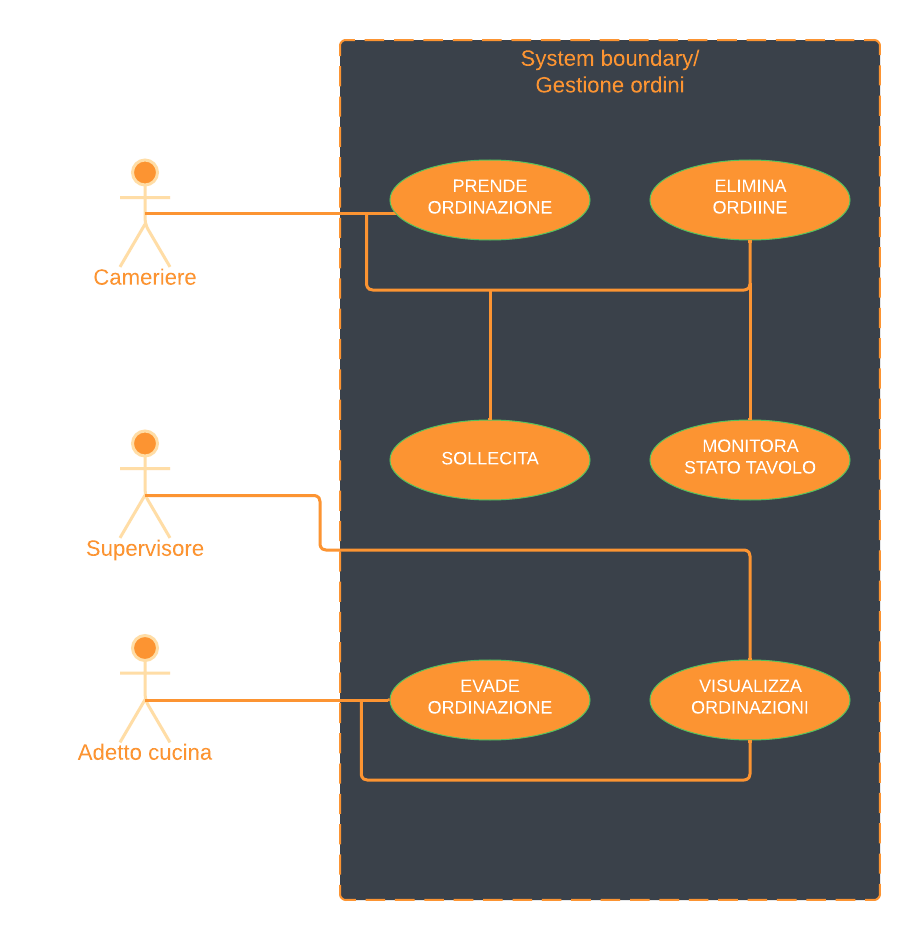
\includegraphics[width=0.7\textwidth]{assets/diagrammi/Use-Case/Gestione ordini.png}
        \caption{Use Case relativo alla gestione degli ordini}
        \label{fig:ucdOrderMgmt}
    \end{figure}
    
    \begin{figure}[H]
        \centering
        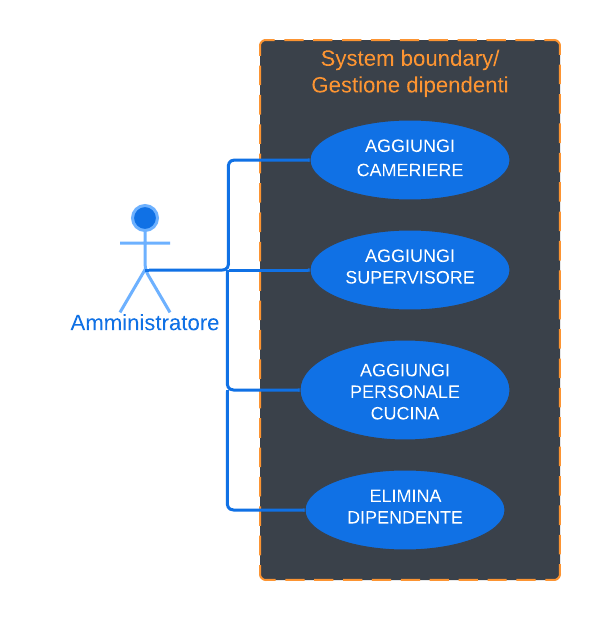
\includegraphics[width=0.6\textwidth]{assets/diagrammi/Use-Case/Gestione dipendenti.png}
        \caption{Use Case relativo alla gestione dei dipendenti}
        \label{fig:ucdWorkersMgmt}
    \end{figure}

    \begin{figure}[H]
        \centering
        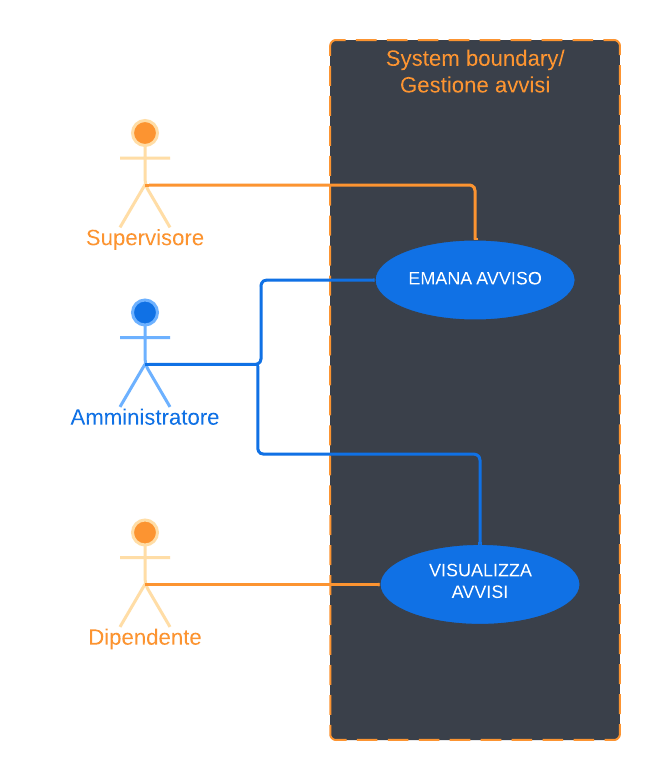
\includegraphics[width=0.8\textwidth]{assets/diagrammi/Use-Case/Gestione avvisi.png}
        \caption{Use Case relativo alla gestione degli avvisi}
        \label{fig:ucdAdvMgmt}
    \end{figure}

\newpage